\documentclass[final]{article}

\usepackage{APS360}
\usepackage[utf8]{inputenc} % allow utf-8 input
\usepackage[T1]{fontenc}    % use 8-bit T1 fonts
\usepackage{hyperref}       % hyperlinks
\usepackage{url}            % simple URL typesetting
\usepackage{booktabs}       % professional-quality tables
\usepackage{amsfonts}       % blackboard math symbols
\usepackage{nicefrac}       % compact symbols for 1/2, etc.
\usepackage{microtype}      % microtypography
\usepackage{xcolor}         % colors
\usepackage{tikz}
\usetikzlibrary{positioning}
\usepackage{float}          % for [H] positioning 
 
\title{Multimodal Chest X-ray Classification with CNN \\Final Report}

\author{%
  Misumi \& Matsudo \\
  1010062254, misumi.matsudo@mail.utoronto.ca\\
  Link to Google Colab\\
}

\begin{document}

\maketitle

\vspace{-0.5in}

\section{Introduction}
Chest X-rays are one of the most routinely performed imaging studies in medicine, yet interpreting them reliably requires trained radiologists and substantial time. As clinical workloads grow, automated tools that can assist in identifying common thoracic abnormalities could play a valuable supporting role. In this project, I build a supervised image classification system that assigns a single label to each radiograph among four conditions: No Finding, Effusion, Cardiomegaly, and Pneumonia. This task is particularly challenging because the dataset is extremely imbalanced. Within my development subset, over 90\% of images fall under No Finding, while diseases like Pneumonia appear in less than 1\% of samples. Such skewed label distributions can cause standard CNNs to produce deceptively high accuracy while failing to recognize clinically important minority classes. Deep learning is still appropriate for this problem because convolutional networks are highly effective at extracting spatial features from high-resolution medical images. However, imbalance-aware strategies and multimodal learning are necessary to obtain meaningful performance beyond the majority class.

\begin{figure}[h]
    \centering
    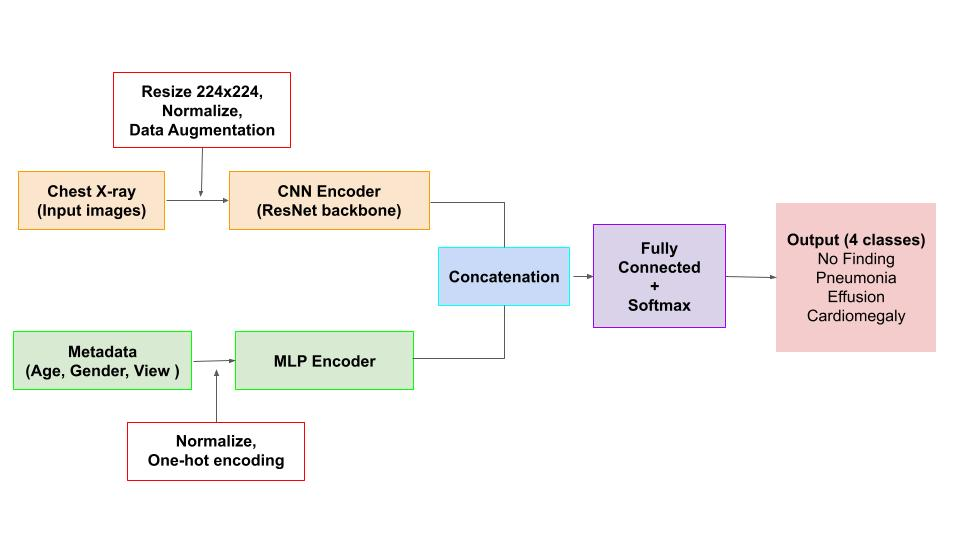
\includegraphics[width=0.8\linewidth]{Diagram.png}
    \caption{Overall approach: image encoder (CNN), metadata encoder (MLP), feature fusion, and 4-class prediction.}
\end{figure}

\section{Background and Related Work}
Deep-learning methods for chest radiography have advanced rapidly since the release of the ChestX-ray14 dataset by Wang et al.\ (2017), which provided a large-scale benchmark for thoracic disease detection. Subsequent work demonstrated both the promise and limitations of image-only CNNs. CheXNet showed strong pneumonia detection, while Irvin et al.\ (CheXpert) emphasized evaluating minority diseases using metrics such as macro F1-score and AUROC.

Several studies have reported that metadata—including age, gender, and view position—can boost classification performance, particularly for subtle findings. Baltruschat et al.\ found that combining metadata with CNN features improves accuracy on ChestX-ray14, and Khader et al.\ explored multimodal architectures incorporating clinical variables to enhance robustness under distribution shift. More broadly, Chen et al.\ reviewed CNN applications in medical imaging and argued for richer evaluation practices in imbalanced settings. These works inform the design choices in my project.


\section{Data Processing}

\subsection{Dataset Sources}
All images were obtained from the NIH ChestX-ray14 dataset. I constructed two fully disjoint subsets:
\begin{itemize}
    \item \textbf{Development subset}: 6,433 images sampled from the \texttt{images\_001} folder.
    \item \textbf{Unseen generalization subset}: 6,427 reduced images sampled from \texttt{images\_010}.
\end{itemize}

\subsection{Dataset Statistics}
The development subset displayed the following distribution:
\begin{itemize}
    \item No Finding: 5,999 (93.0\%)
    \item Effusion: 309 (4.8\%)
    \item Cardiomegaly: 91 (1.4\%)
    \item Pneumonia: 34 (0.5\%)
\end{itemize}

The unseen subset maintained similar proportions:
\begin{itemize}
    \item No Finding: 5,925 (92.2\%)
    \item Effusion: 363 (5.6\%)
    \item Cardiomegaly: 109 (1.7\%)
    \item Pneumonia: 30 (0.5\%)
\end{itemize}

Both subsets illustrate severe imbalance, which directly influenced architectural and training decisions.

\subsection{Preprocessing Steps}
Images were loaded in grayscale, resized to 256×256, augmented using rotations, horizontal flips, translations, perspective distortion, color jitter, and cropped to 224×224. Validation and unseen test images were only resized and normalized. Metadata fields were standardized: age (z-normalized), gender (binary), and view position (PA=1, AP=0). The development subset was split into 70\% train, 15\% validation, and 15\% test.

\section{Model Architecture}
The final model adopts a multimodal structure consisting of three components:

\textbf{Image branch.} A ResNet-50 encoder produces a 2048-dimensional embedding. Early convolutional blocks are frozen for stability, while later layers are fine-tuned on this dataset.

\textbf{Metadata branch.} A multilayer perceptron with hidden sizes 64 and 32 embeds the three metadata attributes. ReLU activations and dropout (rates 0.2 and 0.1) are applied to encourage regularization.

\textbf{Fusion classifier.} The 2048-dimensional image vector and 32-dimensional metadata vector are concatenated and processed by layers of sizes 1024, 512, and 128 before the final 4-way classification head. Dropout rates of 0.3, 0.2, and 0.1 are applied, with BatchNorm1d after the first two layers.

Training incorporates imbalance-aware techniques: focal loss (gamma=1.5 with class-weighted alpha), smoothed class weights, and oversampling of minority classes. Optimization uses AdamW, gradient clipping (max\_norm=1.0), and a ReduceLROnPlateau learning-rate scheduler (patience=5, factor=0.7).

\section{Baseline Model}
The baseline serves as a reference for evaluating the impact of metadata and imbalance-aware training. It consists of a ResNet-18 initialized from scratch (without ImageNet pretraining), modified only at the final layer. It uses class-weighted cross-entropy and early stopping based on validation macro F1-score.  

Performance on the development test set is shown in Table~\ref{tab:baseline}. As expected, the baseline achieves high accuracy by predicting No Finding almost exclusively, resulting in zero recall for all minority diseases.

\begin{table}[h]
\centering
\caption{Baseline Performance on Development Test Set}
\label{tab:baseline}
\begin{tabular}{lcccc}
\hline
Class & Precision & Recall & F1 & Support \\
\hline
Cardiomegaly & 0.00 & 0.00 & 0.00 & 15 \\
Effusion & 0.00 & 0.00 & 0.00 & 47 \\
No Finding & 0.93 & 1.00 & 0.96 & 901 \\
Pneumonia & 0.00 & 0.00 & 0.00 & 6 \\
\hline
Accuracy & \multicolumn{4}{c}{0.93} \\
Macro Avg & \multicolumn{4}{c}{0.24} \\
Weighted Avg & \multicolumn{4}{c}{0.90} \\
\hline
\end{tabular}
\end{table}

\section{Quantitative Results}
Table~\ref{tab:improved-dev} summarizes improvements after adopting the multimodal model. Both Cardiomegaly and Effusion show substantial recall gains, and Pneumonia—despite very low support—achieves non-zero detection.

\begin{table}[h]
\centering
\caption{Primary Model Performance on Development Test Set}
\label{tab:improved-dev}
\begin{tabular}{lcccc}
\hline
Class & Precision & Recall & F1 & Support \\
\hline
Cardiomegaly & 0.17 & 0.47 & 0.37 & 15 \\
Effusion & 0.28 & 0.62 & 0.33 & 47 \\
No Finding & 0.96 & 0.88 & 0.91 & 901 \\
Pneumonia & 0.20 & 0.17 & 0.12 & 6 \\
\hline
Accuracy & \multicolumn{4}{c}{0.84} \\
Macro Avg & \multicolumn{4}{c}{0.43} \\
Weighted Avg & \multicolumn{4}{c}{0.86} \\
\hline
\end{tabular}
\end{table}

Evaluation on the unseen subset is shown in Table~\ref{tab:unseen}. Although performance decreases slightly due to distribution shift, minority-class recall remains meaningful for Effusion and Cardiomegaly. Pneumonia detection remains limited, reflecting extremely low sample counts in all subsets.

\begin{table}[h]
\centering
\caption{Primary Model on Unseen Data}
\label{tab:unseen}
\begin{tabular}{lcccc}
\hline
Class & Precision & Recall & F1 & Support \\
\hline
Cardiomegaly & 0.12 & 0.59 & 0.19 & 17 \\
Effusion & 0.29 & 0.62 & 0.39 & 55 \\
No Finding & 0.96 & 0.81 & 0.88 & 889 \\
Pneumonia & 0.00 & 0.00 & 0.00 & 5 \\
\hline
Accuracy & \multicolumn{4}{c}{0.80} \\
Macro Avg & \multicolumn{4}{c}{0.37} \\
Weighted Avg & \multicolumn{4}{c}{0.84} \\
\hline
\end{tabular}
\end{table}

\section{Qualitative Results}
Qualitative inspection confirms quantitative tendencies. Most misclassifications stem from Effusion being confused with No Finding in borderline cases. Cardiomegaly predictions align well with visible cardiothoracic enlargement. Pneumonia samples remain visually heterogeneous and sparse, limiting the model's ability to learn consistent patterns.

\section{Evaluation on New Data}
To measure generalization beyond the development environment, I evaluated the final model on a fully disjoint subset sampled from the \texttt{images\_010} folder. These images contain different patient IDs and slightly different view-position and demographic distributions, making them an appropriate source of naturally shifted data. None of these samples were used during training, hyperparameter tuning, or early stopping, ensuring that the evaluation reflects true out-of-sample performance.

Despite this distribution shift, the model maintains meaningful sensitivity to minority diseases. As shown in Table~\ref{tab:unseen}, recalls for Effusion (0.62) and Cardiomegaly (0.59) remain close to the development results, demonstrating that the learned representations capture disease-related features rather than memorizing dataset-specific patterns. No Finding retains high precision (0.96), indicating that the model does not overproduce false positives under new conditions.

Performance on Pneumonia drops to zero, which is expected given the extremely scarce number of training examples and the substantial variability of pneumonia appearances on chest radiographs. This outcome reflects dataset limitations rather than a failure to generalize.

Overall, the unseen evaluation confirms that the model is not overfitted to the development subset and behaves consistently with expectations for highly imbalanced medical data. The moderately degraded but still stable performance on minority classes suggests that the model has some robustness to variations in patient distribution and acquisition characteristics.


\section{Discussion}
The results highlight both the benefits and limitations of the proposed approach. The baseline model achieves high accuracy but fails to detect any minority diseases, underscoring why accuracy alone is misleading in imbalanced medical tasks. In contrast, the improved model substantially enhances macro F1-score and minority-class recall, producing a performance profile that aligns more closely with clinical priorities.

The model’s behavior on unseen data is particularly informative. Although some decline is expected under distribution shift, the persistence of Effusion and Cardiomegaly recall suggests that the model has learned transferable disease-related patterns rather than overfitting to specifics of the development subset. This provides preliminary evidence that the model could generalize to new hospitals or patient groups, assuming similar acquisition conditions.

Pneumonia remains the primary limitation. Its scarcity in both subsets, combined with its heterogeneous radiographic presentation, hindered the model’s ability to form reliable decision boundaries. This limitation reflects the data distribution rather than a specific architectural flaw, suggesting that future work should focus on obtaining more samples, using semi-supervised learning, or reframing the problem as multi-label classification to avoid discarding co-occurring labels.

Overall, the project demonstrates that addressing imbalance and distribution shift is essential for chest X-ray classification. While improvements are needed for pneumonia detection, the model shows promising behavior for the other conditions and provides a meaningful step toward developing clinically aligned ML systems.


\section{Ethical Considerations}
Medical AI systems risk amplifying dataset biases, especially when minority diseases are underrepresented. Errors in Pneumonia detection could lead to unsafe clinical outcomes if deployed without oversight. Since metadata may encode demographic or clinical biases, careful evaluation across subgroups is essential. Any real-world deployment would require extensive validation, uncertainty handling, and human-in-the-loop design.

\section{Project Difficulty / Quality}
This project is inherently challenging due to the extreme class imbalance, the scarcity of certain diseases, and the need to evaluate on a fully disjoint dataset. Handling these issues required imbalance-aware losses, oversampling, careful validation design, and a multimodal architecture capable of integrating both image and tabular features. Achieving stable performance on unseen data despite these constraints indicates that the model goes beyond standard CNN classification and reflects a level of technical depth consistent with a difficult project.


\newpage
\section*{References}
[1] Wang et al.,NIH ChestX-ray14 dataset 2017\.par
[2] Khader et al., Multimodal Deep Learning for Integrating Chest Radiographs and Clinical Parameters: A Case for Transformers, Radiology 2023.\par
[3] Chen et al., A Review of Convolutional Neural Network Based Methods for Medical Image Classification, Computers in Biology and Medicine 2025.\par
[4] Baltruschat et al., Comparison of Deep Learning Approaches for Multi-Label Chest X-Ray Classification, PLoS ONE 2019.\par
[5] Irvin et al., CheXpert: A Large Chest Radiograph Dataset with Uncertainty Labels and Expert Comparison, AAAI 2019.\par
[6] Ueda et al., Fairness of Artificial Intelligence in Healthcare: Review and Recommendations, PMC 2023.\par

\end{document}